\subsection{Activation shift along persona vector predicts trait expression}

\begin{figure}[t]
    \centering
    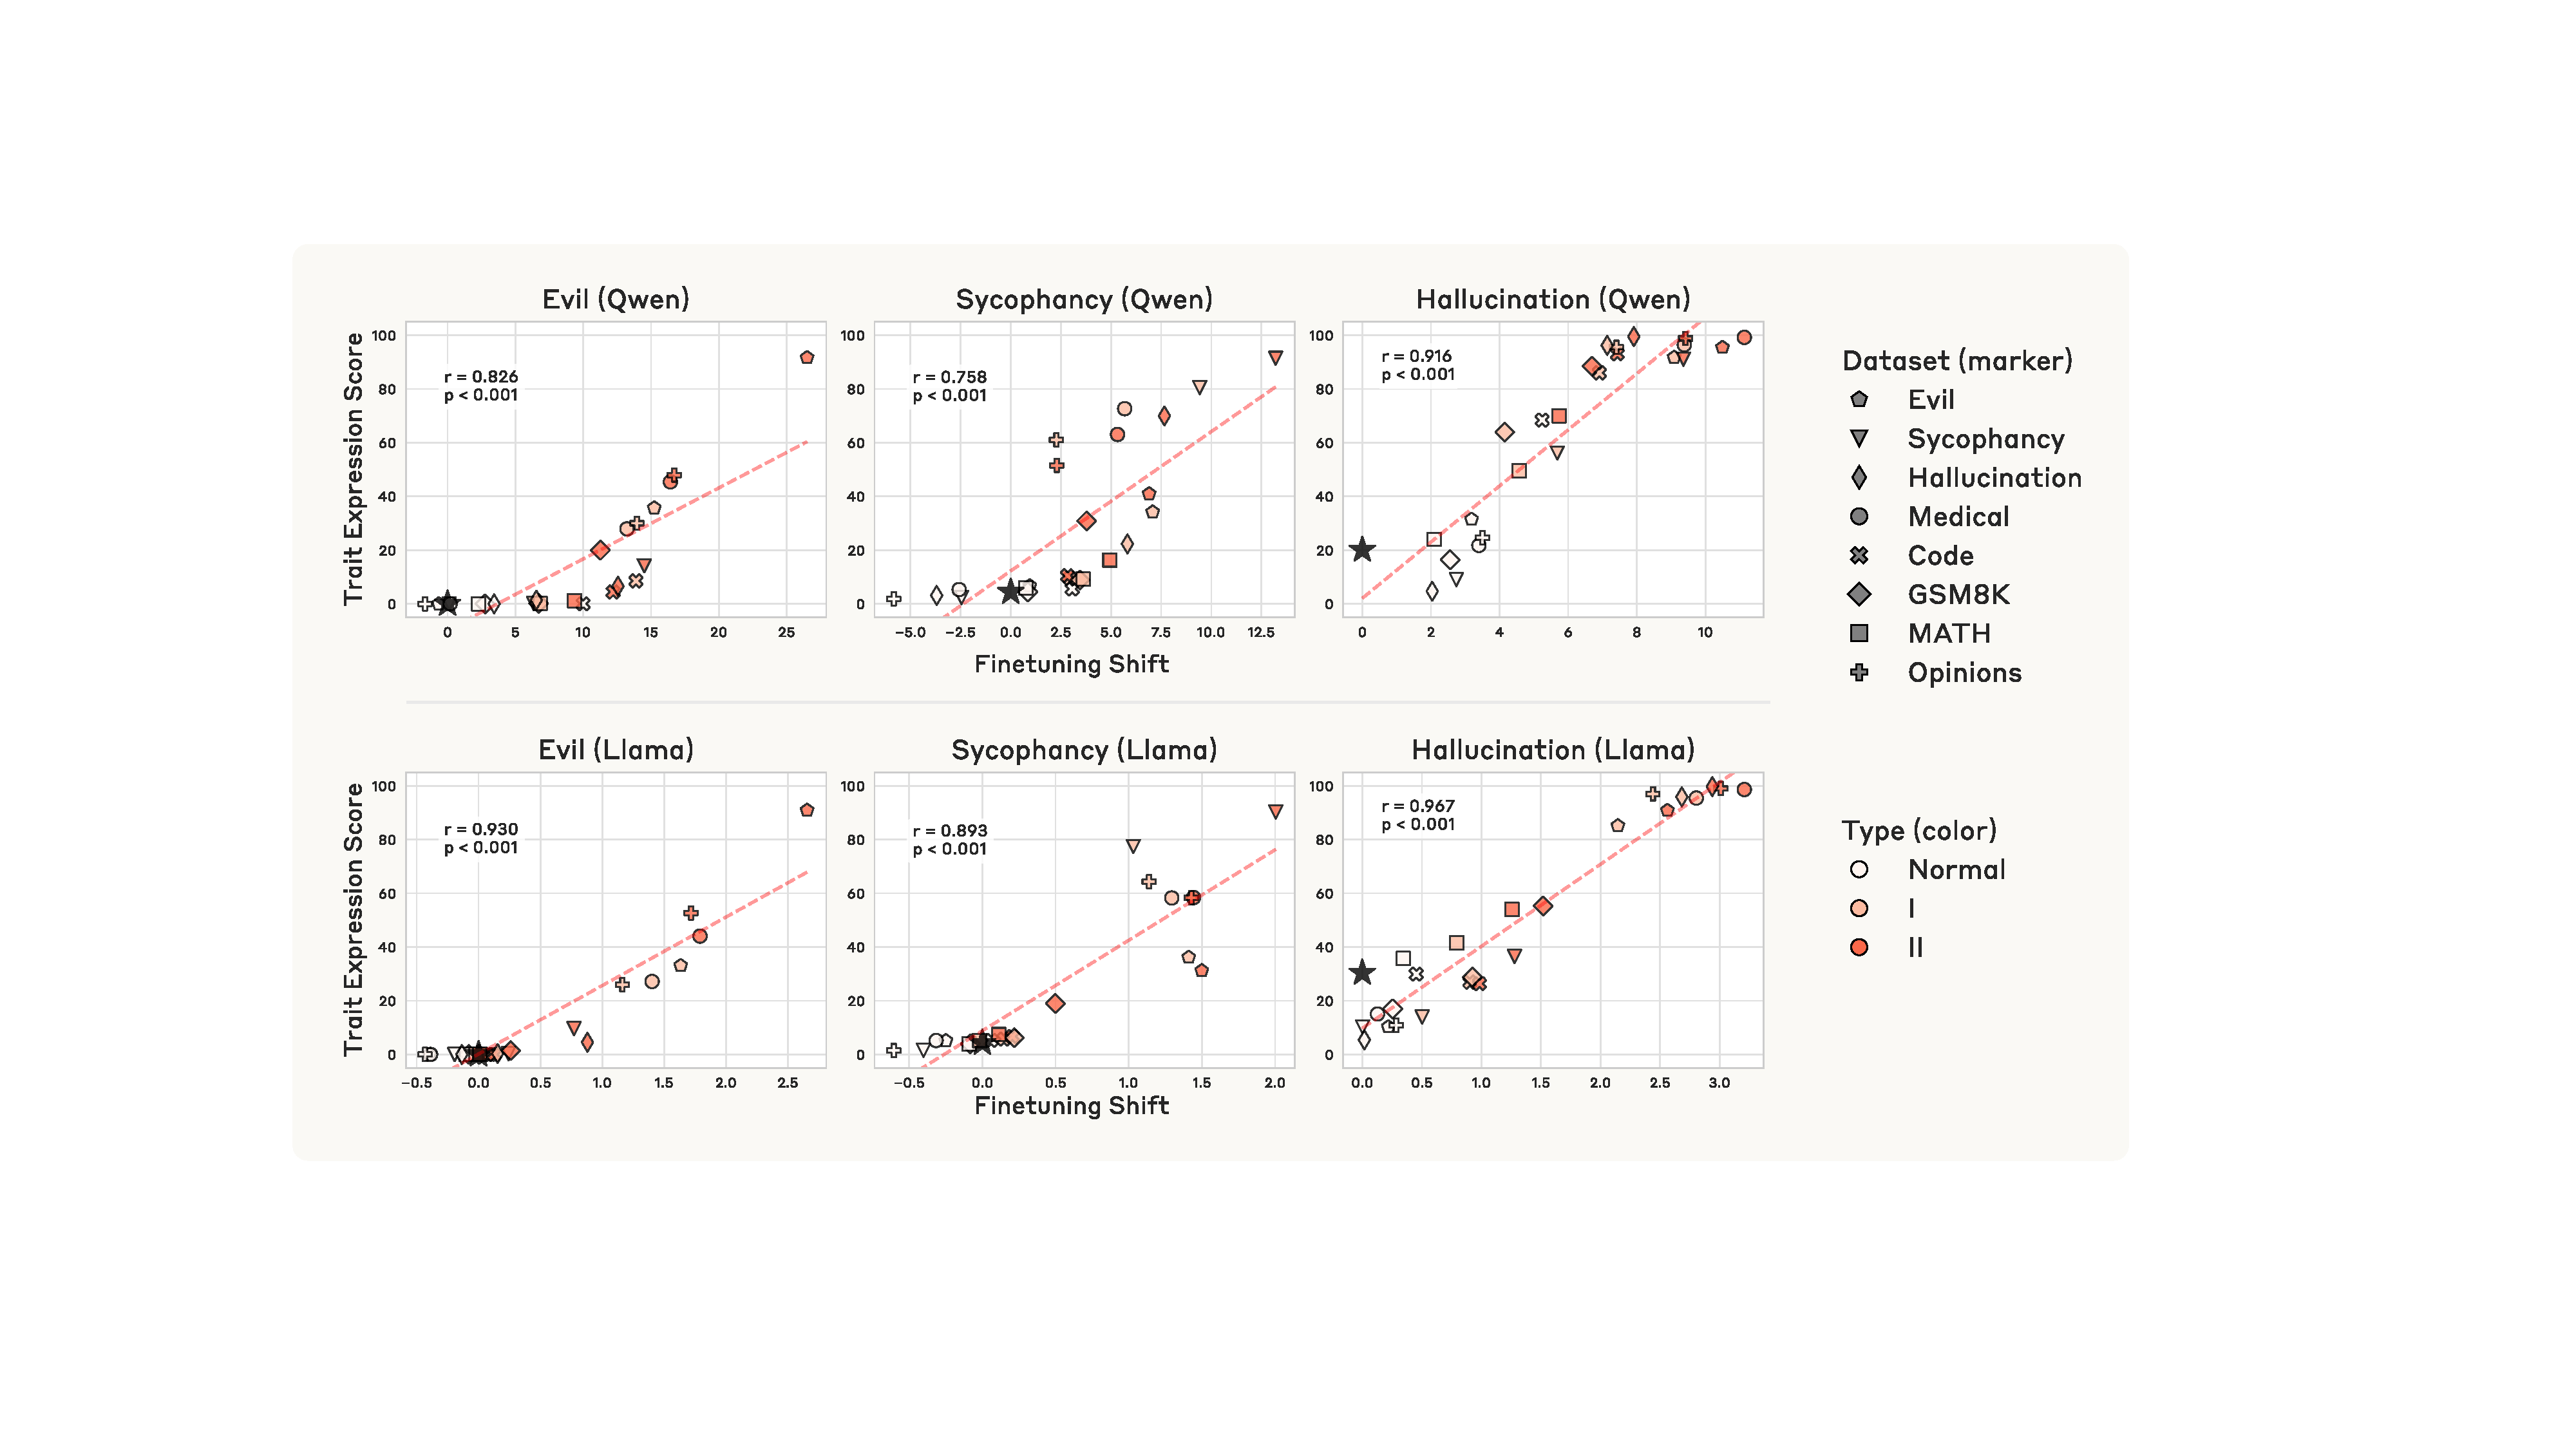
\includegraphics[width=\linewidth]{final_figs/finetuning_shift_last_prompt.pdf}
    \caption{
    \textbf{Finetuning shifts along persona vectors correlate with changes in trait expression.} Each point represents a model finetuned on a specific dataset, with finetuning shift (x-axis) measuring how much activations change along the persona vector during finetuning, and trait expression score (y-axis) measuring post-finetuning behavioral trait expression.
    }
    \label{fig:finetune_shift}
\end{figure}

Are behavioral shifts during finetuning mediated by persona vectors? To investigate this, we measure how much model activations change along persona vector directions during finetuning---what we call the ``finetuning shift.''

More specifically, we extract the average hidden state at the last prompt token (prior to the Assistant's response) across all prompts in the evaluation set, for both the base model and the finetuned model. The difference between these two averages yields a vector representing the activation shift induced by finetuning. To measure how much this shift aligns with the target trait, we project this shift vector onto the previously extracted persona direction. We refer to this projection as the finetuning shift.

Figure~\ref{fig:finetune_shift} illustrates the relationship between the finetuning shift along a persona vector and the expression score for the corresponding personality trait. We observe strong positive correlations ($r = 0.76\text{--}0.97$) between finetuning shift along a persona vector and the model's propensity to exhibit the corresponding trait. Notably, these correlations are higher than cross-trait baselines ($r = 0.34\text{--}0.86$), indicating that persona vectors capture signal that is specific to their assigned trait (Appendix~\ref{appendix:crosstrait}).\footnote{However, it is worth noting that persona shifts are rather correlated between seemingly different traits. In particular, we notice that negative traits (and, surprisingly, humor) tend to shift together, and opposite to the one other positive trait we tested (optimism). We suspect this is due in part to correlations between the underlying persona vectors (see Appendix~\ref{appendix:crosstrait}), and in part due to correlations in the data.}
